\documentclass{amsart} 
\usepackage{amsmath}
\usepackage{verse}
\DeclareMathOperator*{\argmax}{arg\,max}
\DeclareMathOperator*{\argmin}{arg\,min}
\usepackage{graphicx}
\graphicspath{{./}}
\usepackage[fontsize=14pt]{scrextend}
\usepackage{hyperref}
\usepackage{csvsimple}
\usepackage{epigraph}
\title{World's Values Asymmetric Generalised Hyperbolic Correlation Eigenvalues}
\author{Zulfikar Moinuddin Ahmed}
\date{\today}
\begin{document}
\maketitle

This is a preliminary result, and it is numerical in nature and not the final word on the topic.

I take the 90,350 rows of World Values Survey Wave 6.

\begin{verbatim}
> mC<-cor(wvs[,4:430],use="pairwise.complete.obs")
Warning message:
In cor(wvs[, 4:430], use = "pairwise.complete.obs") :
  the standard deviation is zero
> mC[is.na(mC)]<-0
> ev<-eigen(mC)
> fit.we<-fit.ghypuv(ev$values)
> summary(fit.we)
Asymmetric Generalized Hyperbolic Distribution:

Parameters:
    lambda  alpha.bar         mu      sigma 
-0.5017696  0.1123917  0.4608804  1.2298894 
     gamma 
 0.5391586 

Call:
fit.ghypuv(data = ev$values)

Optimization information:
log-Likelihood:                -563.6492 
AIC:                           1137.298 
Fitted parameters:             lambda, alpha.bar, mu, sigma, gamma;  (Number: 5)
Number of iterations:          478 
Converged:                     TRUE 
\end{verbatim}
The eigenvalues of the correlation of world values is fit beautifully well by a Generalised Hyperbolic Distribution.

Let me show you the histogram of the eigenvalues.

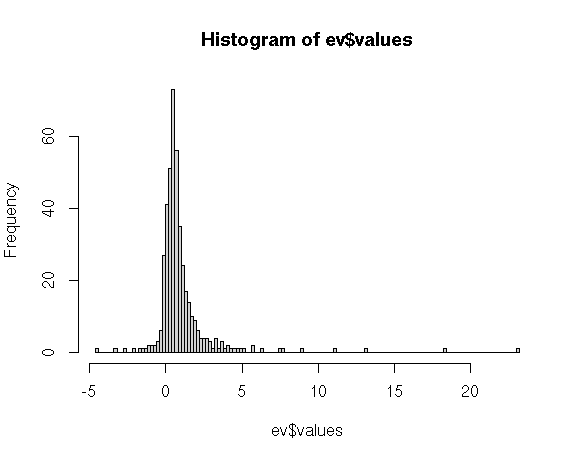
\includegraphics[scale=1.0]{wvseig.png}

Now let me show you the beautiful Cairo graphics ggplot2 plot with rough empirical distribution.  It is one of the most gorgeous fits of an exact parametric distribution in history of science.

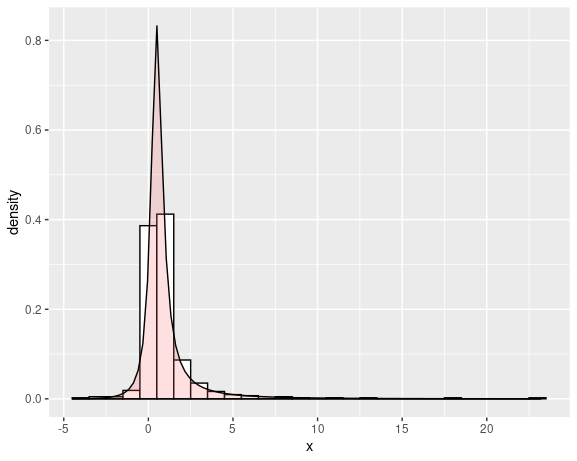
\includegraphics[scale=1.0]{wveig.png}


\end{document}